\documentclass[11pt]{article}
\usepackage[utf8]{inputenc}
\usepackage{geometry}
\geometry{a4paper}
\usepackage{graphicx}
\usepackage{booktabs} 
\usepackage{array} 
\usepackage{paralist}
\usepackage{verbatim}

%\usepackage{subfig}
\usepackage{tikz}
\usepackage{amsmath,bm}
\usepackage{mathrsfs}
\usetikzlibrary{calc}
\usepackage{amssymb}
\usepackage{nccmath}
\usepackage{fancyhdr} 
\pagestyle{fancy} 
\renewcommand{\headrulewidth}{0pt}
\lhead{}\chead{}\rhead{}
\lfoot{}\cfoot{\thepage}\rfoot{}

\usepackage{titling}
\setlength{\droptitle}{-5em}   % This is your set screw

%\numberwithin{equation}{section}

\newcommand{\ra}[1]{\renewcommand{\arraystretch}{#1}}

\usepackage{etoolbox}
 \usepackage{relsize}

\usepackage{tikz,pgfplots}
\usepackage{tikz-3dplot}
\usetikzlibrary{shapes,calc,positioning}
\tdplotsetmaincoords{70}{120}
\usetikzlibrary{patterns}
\usepackage{parskip}

\usepackage{subcaption}

\usepackage{sectsty}
\sectionfont{\fontsize{12}{15}\selectfont}
%\allsectionsfont{\sffamily\mdseries\upshape} % (See the fntguide.pdf for font help)
% (This matches ConTeXt defaults)

%%% ToC (table of contents) APPEARANCE
\usepackage[nottoc,notlof,notlot]{tocbibind} % Put the bibliography in the ToC
\usepackage[titles,subfigure]{tocloft} % Alter the style of the Table of Contents
\renewcommand{\cftsecfont}{\rmfamily\mdseries\upshape}
\renewcommand{\cftsecpagefont}{\rmfamily\mdseries\upshape} % No bold!

%\usepackage[compact]{titlesec}         % you need this package
%\titlespacing{\section}{2pt}{2pt}{2pt} % this reduces space between (sub)sections to 0pt, for example

\usepackage{pgfplots}
    % define a command which stores all commands that are needed for every
    % `raw gnuplot' call
    \newcommand*\GnuplotDefs{
        % set number of samples
        set samples 501;
        %
        % define beta distribution function
        % (copied from <http://gnuplot.sourceforge.net/demo/prob.5.gnu>)
        Binv(p,q)=exp(lgamma(p+q)-lgamma(p)-lgamma(q));
        beta(x,p,q)=p<=0||q<=0?1/0:x<0||x>1?0.0:Binv(p,q)*x**(p-1.0)*(1.0-x)**(q-1.0);
    }

%Regular lowercase Latin
\renewcommand{\a}{\textrm{a}}
\renewcommand{\b}{\textrm{b}}
\renewcommand{\c}{\textrm{c}}
\renewcommand{\d}{\textrm{d}}
\newcommand{\e}{\textrm{e}}
\newcommand{\f}{\textrm{f}}
\newcommand{\g}{\textrm{g}}
\newcommand{\h}{\textrm{h}}
\renewcommand{\i}{\textrm{i}}
\renewcommand{\j}{\textrm{j}}
\renewcommand{\k}{\textrm{k}}
\renewcommand{\l}{\textrm{l}}
\newcommand{\m}{\textrm{m}}
\newcommand{\n}{\textrm{n}}
\renewcommand{\o}{\textrm{o}}
\newcommand{\p}{\mathbf{p}}
\newcommand{\q}{\textrm{q}}
\renewcommand{\r}{\textrm{r}}
\newcommand{\s}{\mathrm{s}}
\renewcommand{\t}{\textrm{t}}
\renewcommand{\u}{\textrm{u}}
\renewcommand{\v}{\textrm{v}}
\newcommand{\w}{\textrm{w}}
\newcommand{\x}{\textrm{x}}
\newcommand{\y}{\textrm{y}}
\newcommand{\z}{\textrm{z}}

%Regular uppercase latin
\newcommand{\A}{\mathrm{A}}
\newcommand{\C}{\mathrm{C}}
\newcommand{\D}{\mathrm{D}}
\newcommand{\F}{\mathrm{F}}
\newcommand{\I}{\mathrm{I}}
\renewcommand{\P}{\mathrm{P}}
\newcommand{\Q}{\mathrm{Q}}
\newcommand{\R}{\mathrm{R}}
\renewcommand{\S}{\mathrm{S}}
\renewcommand{\H}{\mathrm{H}}
\newcommand{\W}{\mathrm{W}}
\renewcommand{\L}{\mathrm{L}}
\newcommand{\E}{\mathrm{E}}
\newcommand{\T}{\mathrm{T}}
\newcommand{\N}{\mathrm{N}}
\newcommand{\X}{\mathrm{X}}
\newcommand{\U}{\mathrm{U}}
\newcommand{\V}{\mathrm{V}}

%Bold lowercase Latin
\newcommand{\bb}{\mathbf{b}}
\newcommand{\bc}{\mathbf{c}}
\newcommand{\bd}{\mathbf{d}}
\newcommand{\be}{\mathbf{e}}
\renewcommand{\bf}{\mathbf{f}}
\newcommand{\br}{\mathbf{r}}
\newcommand{\bs}{\mathbf{s}}
\newcommand{\bu}{\mathbf{u}}
\newcommand{\bx}{\mathbf{x}}
\newcommand{\by}{\mathbf{y}}
\newcommand{\ba}{\mathbf{a}}
\newcommand{\bn}{\mathbf{n}}
\newcommand{\bt}{\mathbf{t}}
\newcommand{\bq}{\mathbf{q}}
\newcommand{\bw}{\mathbf{w}}
\newcommand{\bv}{\mathbf{v}}

\newcommand{\byk}{\boldsymbol{\nu}}
\newcommand{\bxk}{\boldsymbol{\mu}}

%Bold uppercase Latin
\newcommand{\bA}{\mathbf{A}}
\newcommand{\bB}{\mathbf{B}}
\newcommand{\bC}{\mathbf{C}}
\newcommand{\bD}{\mathbf{D}}
\newcommand{\bI}{\mathbf{I}}
\newcommand{\bK}{\mathbf{K}}
\newcommand{\bL}{\mathbf{L}}
\newcommand{\bN}{\mathbf{N}}
\newcommand{\bS}{\mathbf{S}}
\newcommand{\bH}{\mathbf{H}}
\newcommand{\bX}{\mathbf{X}}
\newcommand{\bU}{\mathbf{U}}
\newcommand{\bF}{\mathbf{F}}
\newcommand{\bE}{\mathbf{E}}
\newcommand{\bY}{\mathbf{Y}}
\newcommand{\bP}{\mathbf{P}}
\newcommand{\bT}{\mathbf{T}}
\newcommand{\bV}{\mathbf{V}}
\newcommand{\bR}{\mathbf{R}}
\newcommand{\bQ}{\mathbf{Q}}

\newcommand{\Grad}{\text{Grad}}
\newcommand{\grad}{\text{grad}}
\renewcommand{\div}{\text{div}}
\newcommand{\Div}{\text{Div}}


%Regular Greek
\newcommand{\eps}{{\varepsilon}}
\newcommand{\sig}{{\sigma}}

%Bold Greek
\newcommand{\beps}{\bm{\varepsilon}}
\newcommand{\bsig}{\bm{\sigma}}
\newcommand{\bchi}{\bm{\chi}}

\newcommand{\balp}{\bm{\alpha}}
\newcommand{\bbet}{\bm{\beta}}

%Time
\newcommand{\dt}{\Delta \mathrm{t}}

%Misc
\renewcommand{\k}{k}
\newcommand{\ks}{\{k\ast\}}
\newcommand{\fk}{\tilde{f}^{\{k\}}}
\newcommand{\dfk}{\tilde{f}^{\{k\}}}
\newcommand{\dfok}{\frac{\partial f_0}{\partial \rho_j} \bigg|_{\brho^{\k}}}
\newcommand{\dflk}{\frac{\partial f_1}{\partial \rho_j}\bigg|_{\brho^{\k}} }
\newcommand{\dtL}{\frac{\partial \tL^{\k}}{\partial \rho_j} }
\newcommand{\dtLam}{\frac{\partial \tL^{\k}}{\partial \lambda} }
\newcommand{\sumjn}{ \stackrel{n}{\underset{j}{\text{\LARGE $\Sigma$}}}}
\newcommand{\sumln}{ \stackrel{n}{\underset{l}{\text{\LARGE $\Sigma$}}}}
\newcommand{\sumkn}{ \stackrel{n}{\underset{k}{\text{\LARGE $\Sigma$}}}}
\newcommand{\sumkd}{ \stackrel{d}{\underset{k}{\text{\LARGE $\Sigma$}}}}
\newcommand{\sumid}{ \stackrel{d}{\underset{i}{\text{\LARGE $\Sigma$}}}}
\newcommand{\sumi}{ \underset{i}{\text{\LARGE $\Sigma$}}}
\newcommand{\blam}{\bm{\lambda}}
\newcommand{\bLam}{\bm{\Lambda}}
\newcommand{\bkap}{\bm{\kappa}}
\newcommand{\bpar}{\bm{\partial}}

\newcommand{\tL}{\tilde{\mathcal{L}}}
\newcommand{\brho}{\bm{\rho}}
\newcommand{\rK}{\mathbf{K}}
\newcommand{\rG}{\mathbf{G}}
\newcommand{\G}{\mathrm{G}}
\newcommand{\Bomega}{\mathbf{\Omega}}
\newcommand{\Bamma}{\mathbf{\Gamma}}


\newcommand{\bips}{\bm{\epsilon}^{\textrm{init}}} %bold strain
\newcommand{\baps}{\bm{\epsilon}^{\star}} %bold strain
\newcommand{\bsid}{\bm{\sigma}^{\dagger}} %bold strain

\newcommand{\bops}{\bm{\epsilon}^{0}} %bold strain
\newcommand{\rE}{\mathrm{E}}
\newcommand{\rF}{\mathrm{F}}
\newcommand{\cF}{\mathcal{F}}


\newcommand{\0}{\mathbf{0}}

\newcommand{\bzet}{\bm{\zeta}} %bold strain
\newcommand{\btau}{\bm{\tau}}

\newcommand{\bvsig}{\bm{\sigma}} %bold stress
\newcommand{\bveps}{\bm{\varepsilon}} %bold strain

\newcommand{\ui}{\textrm{u}_{i}} %index displacement

%\renewcommand{\pi}{\textrm{p}_{i}} %index displacement

\newcommand{\si}{\textrm{s}_{i}} %index displacement

\newcommand{\uij}{\textrm{u}_{i,j}} %index displacement
\newcommand{\uji}{\textrm{u}_{j,i}} %index displacement

\newcommand{\ci}{\textrm{c}_{i}} %index constrained

\newcommand{\epsij}{\varepsilon_{ij}} %index strain
\newcommand{\epskl}{\varepsilon_{kl}} %index strain
\newcommand{\sigij}{\sigma_{ij}} %index stress

\newcommand{\sigijj}{\sigma_{ij,j}} %index stress

\newcommand{\nj}{\textrm{n}_j} %normal
\newcommand{\ti}{\textrm{t}_i} %traction

\newcommand{\wkl}{w_{kl}} %index displacement

\newcommand{\wij}{w_{ij}} %index displacement
\newcommand{\mij}{m_{ij}} %index displacement
\newcommand{\mijj}{m_{ij,j}} %index displacement
\newcommand{\vi}{v_{i}} %index displacement
\newcommand{\ri}{r_{i}} %index displacement
\renewcommand{\vi}{v_{i}} %index displacement
\newcommand{\yi}{y_{i}} %index displacement

\newcommand{\vij}{v_{i,j}} %index displacement
\newcommand{\vji}{v_{j,i}} %index displacement

\newcommand{\gamt}{\Gamma_{\textrm{p}}} %surface
\newcommand{\gamc}{\Gamma_{\textrm{c}}} %surface

\newcommand{\Lijkl}{\mathscr{L}_{ijkl}} %index elas
\newcommand{\bLijkl}{\pmb{\mathscr{{L}}}} %bold elas

\newcommand*\vard{\mathop{}\!\mathrm{d}}


%%%%%%%%%%%%%%%%%%%%%%%%%%%%%%%%%



\makeatletter
\newcommand{\changeoperator}[1]{%
  \csletcs{#1@saved}{#1@}%
  \csdef{#1@}{\changed@operator{#1}}%
}
\newcommand{\changed@operator}[1]{%
  \mathop{%
    \mathchoice{\textstyle\csuse{#1@saved}}
               {\csuse{#1@saved}}
               {\csuse{#1@saved}}
               {\csuse{#1@saved}}%
  }%
}
\makeatother

\changeoperator{sum}
\changeoperator{prod}

\title{An interpretation of Bayesian global optimization as proposed by Snyman and Fatti \cite{snyman1987}}
\author{Dirk Munro (Hamburg, Germany)}
\date{\today } 
% Activate to display a given date or no date (if empty),
         % otherwise the current date is printed 

\begin{document}
\maketitle

\section{Confidence-based global optimization}

Assume that we have an optimization problem and a search algorithm (e.g. gradient-based) to solve it. That is, for a given starting position $\bx_0$ the algorithm will return a stationary point $\bx_\ast$, a candidate optimum from all the potential optima---in general there are plenty of local optima, and one global optimum. 

Assume that the optimization problem has a finite but unknown number of optima $\bx^j_\ast$, with $j=1,2,\ldots, s$, and that from a particular starting point $\bx_0$, the algorithm will converge to one of them. This procedure which transforms a given $\bx_0$ to one of the the optima $\bx^j_\ast$ is deterministic, yet unpredictable. In other words, given a new $\bx_0$ (pulled `from a hat', so to speak), we do not know \emph{a priori} which $\bx^j_\ast$ will be returned; however, given the same $\bx_0$ again, the same $\bx^j_\ast$ (from before) will be returned.

Lets say an an `experiment' consists of sampling a random starting point $\bx_0$ from the design domain, and running the optimization algorithm. There is hence a probability $\P^j_\ast$ that a particular $\bx^j_\ast$ will be returned. Also, there is a probability $\P_\ast$ that the (global) optimum will be returned.

What is the probability $\P_\ast$ of finding the global optimum from a random starting point? If we had an estimate of the total number of optima $s$, then a reasonable estimate may be $1/s$...? Or rather, the flexible form of the Beta distribution may be assumed
\begin{equation}
\label{eqn:beta}
\p[\P_\ast] = \frac{1}{\beta\left[a,b\right]} {\P_\ast}^{a-1}(1 - \P_\ast)^{b-1} \: ,
\end{equation}
which reflects the \emph{probability density function} $\p$ of the probability $\P_\ast$ of finding the global optimum from a random starting position---see for example Figure \ref{fig:beta}. An expected value of $\P_\ast$ given an $a$ and $b$, and other statistical measures, is implied by (\ref{eqn:beta}).
\begin{figure}
\centering
\begin{tikzpicture}
        % define macros which are needed for the axis limits as well as for
        % setting the domain of calculation
        \pgfmathsetmacro{\xmin}{0}
        \pgfmathsetmacro{\xmax}{1}
    \begin{axis}[
        xmin=\xmin,
        xmax=\xmax,
        ymax=10,
        no markers,
        width=14cm,
        height=7cm,
        xlabel = ${\P_\ast}$,
        ylabel = ${\p\left[\P_\ast\right]}$,
        every axis plot/.append style={ultra thick}
    ]
        \addplot gnuplot [raw gnuplot] {
            \GnuplotDefs
            plot [x=\xmin:\xmax] beta(x,1,1);
        };
        \addlegendentry{$a=1$, $b=1$}
        \addplot gnuplot [raw gnuplot] {
            \GnuplotDefs
            plot [x=\xmin:\xmax] beta(x,1,10);
        };
        \addlegendentry{$a=1$, $b=10$}
        \addplot gnuplot [raw gnuplot] {
            \GnuplotDefs
            plot [x=\xmin:\xmax] beta(x,1,100);
        };
        \addlegendentry{$a=1$, $b=100$}
    \end{axis}
\end{tikzpicture}
\caption{\label{fig:beta}Example Beta distributions (probability density functions) of ${\P_\ast}$, for representative values of $a$ and $b$.}
\end{figure}

Bayes' theorem permits us to update the prior probability density function $\p\left[\P_\ast\right]$, given the results from a number of experiments. Assume (for now) that we know the number of `successes' $r$, after a total number of experiments $n$. That is, running the algorithm from $n$ random starting positions, we assume that we can measure the number of times $r$ the global optimum was found ($r$ `successes')\footnote{The severity/subtlety of this assumption---\emph{i.e.}, knowing which is the global optimum, and hence being able to measure the amount of times it is found---is addressed later.}. Given $n$ and $r$, the prior probability density function of $\P_\ast$ may be updated as per Bayes 
\begin{equation}
\label{eqn:bay}
\p[\P_\ast \: | \left[ n, r \right]] = \p\left[ r \: | \left[ n, \P_\ast \right]  \right] \p\left[ \P_\ast \right] \bigg/ \int_0^1 \p\left[ r \: | \left[ n, \P_\ast \right]  \right] \p\left[ \P_\ast \right] \textrm{d}\P_\ast \:
\end{equation}

The new term $\p\left[ r \: | \left[ n, \P_\ast \right]  \right]$ is the probability density function of the number of `successes' $r$, given $n$ experiments and a prior probability $\P_\ast$. This probability density function is thus of the binomial form
\begin{equation}
\label{eqn:binom}
\p\left[ r \: | \left[ \P_\ast , n \right] \right] = \frac{n!}{r! (n - r)!} {\P_\ast}^r ( 1 - \P_\ast)^{n - r} \: .
\end{equation}

In the end, we want to have a measure of confidence in whether we may have found the (global) optimum of the optimization problem, given $n$ experiments, $r$ `successes', and the prior $\P_\ast$. On the one hand, this can be expressed as the probability of having found the true optimum \emph{at least once}, given $n$ and $\P_\ast$ 
\begin{equation}
\label{eqn:al1}
\P \left[ r_\ast \ge 1 | \left[ n, \P_\ast \right] \right] = 1- (1 - \P_\ast)^n \:,
\end{equation}
which follows from the binomial distribution (\ref{eqn:binom}) of the complementary probability: 1 minus the probability of not finding the true optimum at all ($r=0$, after $n$ experiments). On the other hand, we have a probability density function $\p\left[\P_\ast | \left[ n, r \right] \right]$, updated with the results $r$ of $n$ experiments, as per Bayes' theorem (\ref{eqn:bay}). Applying a change-of-variable \cite{dekking2005} to $\p\left[P_\ast | \ldots\right]$ from Eq. (\ref{eqn:bay}), with Eq. (\ref{eqn:al1}) the transformation function, the probability of having found the optimum at least once, in terms of $n$ and $r$, is
\begin{equation}
\label{eqn:al2}
\P \left[ r_\ast \ge 1 | \left[ n, r \right] \right] = \int^1_0 \P \left[ r_\ast \ge 1 | \left[ n, \P_\ast \right] \right] \p\left[\P_\ast | \left[ n, r \right] \right] \textrm{d}P_\ast \:.
\end{equation}

Now, the issue of being able to count the number of `successes' $r_\ast$ from $n$ experiments is addressed. The objective value of a particular optima may be evaluated, $\F \left[ \bx^j_\ast \right]$, and values amongst different optima may be compared: \emph{e.g.} is $\F \left[ \bx^c_\ast \right]$ a better optima than $\F \left[ \bx^d_\ast \right]$? Hence, from $n$ experiments, we can determine what was relatively the best optimum solution found $\bchi_\ast$, and we can count how many solutions $\rho_\ast$ (`relative successes') correspond to this $\bchi_\ast$. If we assume that the probability of finding the global optimum from a random starting point $\P_\ast$, is \emph{at least} the probability of finding any other $\P^j_\ast$
\begin{equation}
\P_\ast \ge \P^j_\ast \: \forall \: j \:,
\end{equation}
then it follows that
\begin{equation}
\P \left[ r_\ast \ge 1 | \left[ n, r \right] \right] \ge \P \left[ \rho_\ast \ge 1 | \left[ n, r \right] \right] \: .
\end{equation}
That is, the probability of having had at least one absolute `success' $r_\ast$, after $n$ experiments, is greater than the probability of having at least one `relative success' $\rho_\ast$. This is property that may have to be justified in the optimization algorithm; \emph{e.g.}, move-limits should be sufficiently large?

Substitution of (\ref{eqn:al1}) and (\ref{eqn:bay}) in (\ref{eqn:al2}), and, in turn, substitution of the binomial (\ref{eqn:binom}) and beta (\ref{eqn:beta}) distributions, permits straight-forward cancellations and simplification \cite{snyman1987} to
\begin{multline}
\label{eqn:res}
\P_f = \P \left[ r_\ast \ge 1 | \left[ n, r \right] \right]  \ge \P \left[ \rho_\ast \ge 1 | \left[ n, r \right] \right] = \\  1 - \beta[r+a,2n-r+b]/\beta[r +a,n-r+b] = \frac{\Gamma[n+a+b]\Gamma[2n-r+b]}{\Gamma[2n+a+b]\Gamma[n-r+b]}\:.
\end{multline}

Further cancellations are made in the factorials, and, in numerical terms, the calculation is dealt with as per the Python function given verbatim below. 

In Table \ref{tab:exp} some example calculations are given with a severely pessimistic estimate of $\p[\P_\ast]$, with $a=1$ and $b=1000$ (see Fig. \ref{fig:beta}). 
\begin{table}
\centering
\caption{\label{tab:exp}Example calculations using Eq. (\ref{eqn:res}), with $a=1$ and $b=1000$ in the prior $\p[\P_\ast]$ . }
\begin{tabular}{ll|r|ll|r|ll|r|ll|r|}
$n$  & $r$  & $\P_f$  & $n$   & $r$  & $\P_f$  & $n$    & $r$  & $\P_f$ & $n$    & $r$  & $\P_f$  \\
\hline
10 & 1  & 0.02  & 100 & 1  & 0.16 &  200 & 1  & 0.27  &  1000 & 1  & 0.56\\
10 & 2  & 0.03  & 100 & 2  & 0.23 &  200 & 2  & 0.37 &  1000 & 2  & 0.70 \\
10 & 3  & 0.04 & 100 & 3  & 0.30 &  200 & 3  & 0.46  &  1000 & 3  & 0.80\\
10 & 4  & 0.05  & 100 & 4  & 0.35 &  200 & 4  & 0.54 &  1000 & 4  & 0.87 \\
10 & 5  & 0.06  & 100 & 5  & 0.41 &  200 & 5  & 0.60  &  1000 & 5  & 0.91 \\
10 & 10 & 0.10 & 100 & 10 & 0.62 &  200 & 10 & 0.82 &  1000 & 10 & 0.99
\end{tabular}
\end{table}


We can see how the confidence in having found the global optimum $\P_f$ changes for different values of $n$ and $r$. For example, with 10 experiments ($n$), even if we have a success rate of 1 in 2 ($r=5$), our confidence is about 5 \%.  However, if we do 100 experiments, and we have only between 5 and 10 successes, then the confidence of having found the global optimum increases to about 50\%. This is not bad, given a prior expectation of $\frac{1}{1 + 1000} \approx \frac{1}{1000}$ (0.1 \%). Given 200 experiments, and 10 successes, our confidence increases to a fairly comfortable 80\%, \emph{etc.}.

\begin{minipage}{\linewidth}
\begin{verbatim}
#
def P_f(ni,ri,a,b):
#
#   see Bolton (2004)
#
    tmp=1e0; abar=a+b-1; bbar=b-ri-1
    for i in range(1,ni+1):
        tmp=tmp*(ni+i+bbar)/(ni+i+abar)
#
    return 1e0-tmp
#
\end{verbatim}
\end{minipage}

\section{Applied to simple topology optimization}
Fittingly avoiding the details of the optimization problem, the procedure is tested on the well-known Python implementation of the classical topology optimization problem \cite{sigmund2001m}. The implementation is taken as is, the starting point is set to an array of values, with each individual element sampled from a uniform distribution between the lower and upper bounds of the problem, and the problem is executed 100 times (embarrassingly parallel). Throughout solutions will be characterized/compared based on objective function values and a measure of the number-of-holes' the topology has (a discrete version of a `perimeter' quantity).

Based on a 1\% threshold in the relative objective function values, the best solution---see Figure \ref{fig:top02}---is found $r=33$ times. Based on a 5\% difference in the perimeter quantity, the best solution was found $r=37$ times. (We have been able to visually inspect whether these counts are representative.) Assuming a (horrible) Beta distribution prior with $a=1$ and $b=1000$, there is a 90\% probability that we have found the global optimum\footnote{Note that the particular filtering applied to the standard problem serves to explicitly restrict the number of solutions; we would have more candidate optima and fewer `successes' for a smaller value of the filter\cite{munro2018design}.}.
\begin{figure}
\centering
\begin{subfigure}{0.4\textwidth}
\centering
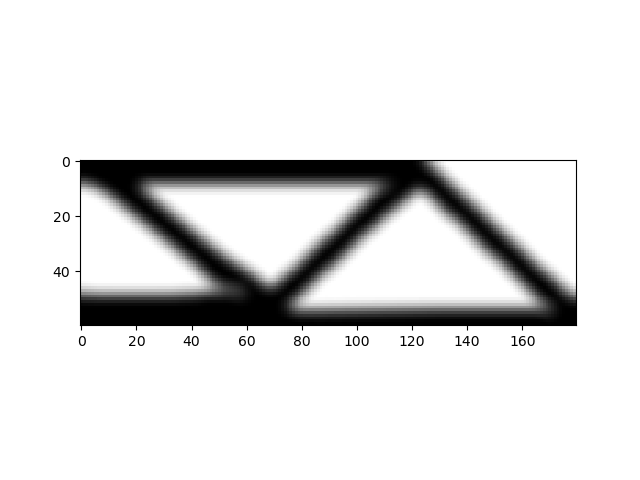
\includegraphics[scale=0.55, trim={2.05cm 4cm 1cm 4cm},clip]{topo_58.png}
\caption{Best solution found \label{fig:glo02}}
\end{subfigure} \hfill
\begin{subfigure}{0.4\textwidth}
\centering
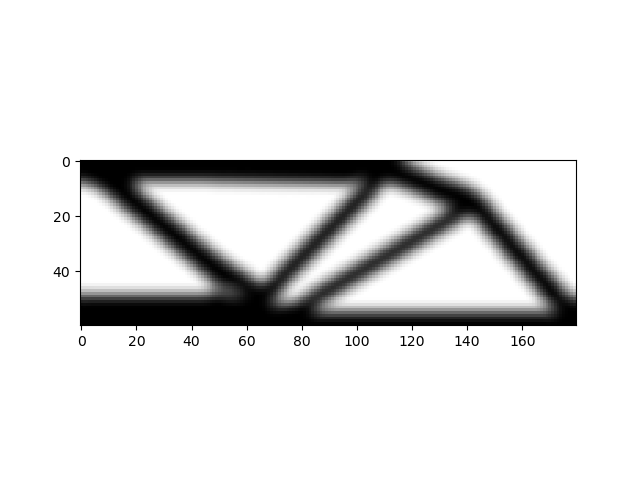
\includegraphics[scale=0.55, trim={2.05cm 4cm 1cm 4cm},clip]{topo_11.png}
\caption{Example of a local optima \label{fig:loc02}}
\end{subfigure}
\caption{Standard/default test problem; $n=100$ experiments. \label{fig:top02}}
\end{figure}

For sake of interest; repeating the 100 experiments with a move-limit of 1.0 in the OC subsolver, results in $r = 60$, almost double the number of `successes'; which brings the probability of having found the global optimum to 99\%. That is, this manner of experimentation may also be a rigorous way of comparing the success of different optimization algorithms and parameter settings---while continuously building up confidence in the best known solution. 

% BIBLIOGRAPHY
\bibliographystyle{unsrt} 
\addcontentsline{toc}{chapter}{References} 
\bibliography{./bib.bib} 
\end{document}
